% 1_introduction.tex

\cleardoublepage
\chapter{Introduction}

  This is where your introduction goes. There will probably be a some references here \parencite{Denman2016a}. The previous citation was done using the \texttt{parencite} command. There is also which the \texttt{textcite} command for in text citations. For instance, \textcite{Colket2001} is a product of the \texttt{textcite} command. Figure~\ref{introduction:specific-impulse} shows you what a figure is. Remember to update the \texttt{graphicspath} in the \texttt{packages.tex} file as you write your thesis.

  \begin{figure}
    \centering
    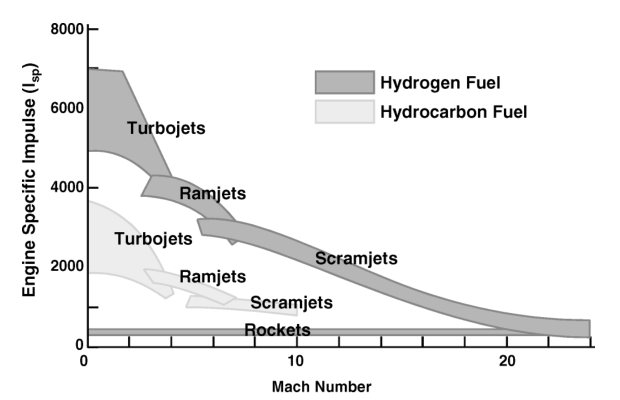
\includegraphics[width=0.8\textwidth]{./figures/1_introduction/specific-impulse}
    \caption{Specific impulse of various engine types for hydrogen and hydrocarbon fuels \parencite{Fry2004}}\label{introduction:specific-impulse}
  \end{figure}

  This template uses the \texttt{nomencl} package. Have a look at the lines below this paragraph in the \texttt{1\_introduction.tex} file to see how this works. Also take a look at lines 21--49 in \texttt{packages.tex} to see the groupings available.
  \nomenclature[r]{$T$}{Static temperature\nomunit{\si{\kelvin}}}
  \nomenclature[r]{$s$}{Entropy\nomunit{\si{\joule\per\kelvin}}}
  \nomenclature[r]{$p$}{Static pressure\nomunit{\si{\pascal}}}
  \nomenclature[g]{$\phi$}{Equivalence ratio\nomunit{-}}

  The remainder of your introduction should include your thesis aim and objectives and a chapter summary.
  
  \section{Research aims}

    The overall aim of this thesis is to

    \begin{quote}
      \emph{make scramjets fly}.
    \end{quote}

    \noindent This will be achieved through the following objectives:

    \begin{enumerate}
      \item \emph{Flying them}\\
      Flying scramjets will conclusively prove that scramjets can fly.

      \item \emph{Fly different types of scramjets}\\
      By flying lots of scramjets we can see that they are awesome. 

      \item \emph{Having 3 objectives is typically good.}\\
      Three objectives just makes this section look complete.
    \end{enumerate}

  \clearpage
  \section{Thesis outline}

    Edit this as required. This thesis is organised in eight chapters which are outlined below. The appendices included at the end of this document contain further technical information and supplementary experimental details. \textcolor{red}{If you want to add colours to the text for some reason (supervisor reviewing etc.), use the \texttt{textcolor} command. Check the code here to see how.}

    \subsubsection*{Chapter 2 - Literature review}

      This chapter presents a review of literature related to the different aspects of this thesis. 

    \subsubsection*{Chapter 3 - Methodology}

      This chapter provides details of the experimental facility, experimental model, and test conditions used in the completion of the experiments that form the majority of this thesis. 

    \subsubsection*{Conclusions}

      The body of this thesis concludes by summarising the most significant findings from Chapters~\ref{chapter:jpp} through~\ref{chapter:numerical}. Recommendations for future studies on cavity flameholders in three-dimensional, hydrocarbon-fuelled scramjet engines, such as the REST engine, are provided.
